\section{Señalamiento original}

    El señalamiento original, ilustrado en la Figura \ref{fig:EJ7_2}, incluye señales de parada próximas a los finales de vías absolutos (S06, S07, S08, S09, S10), señales de maniobras antes de converger en una vía principal (S02, S04, S05) y señales múltiples para cambios de vías divergentes (S01, S03).
    
    \begin{figure}[H]
    	\centering
    	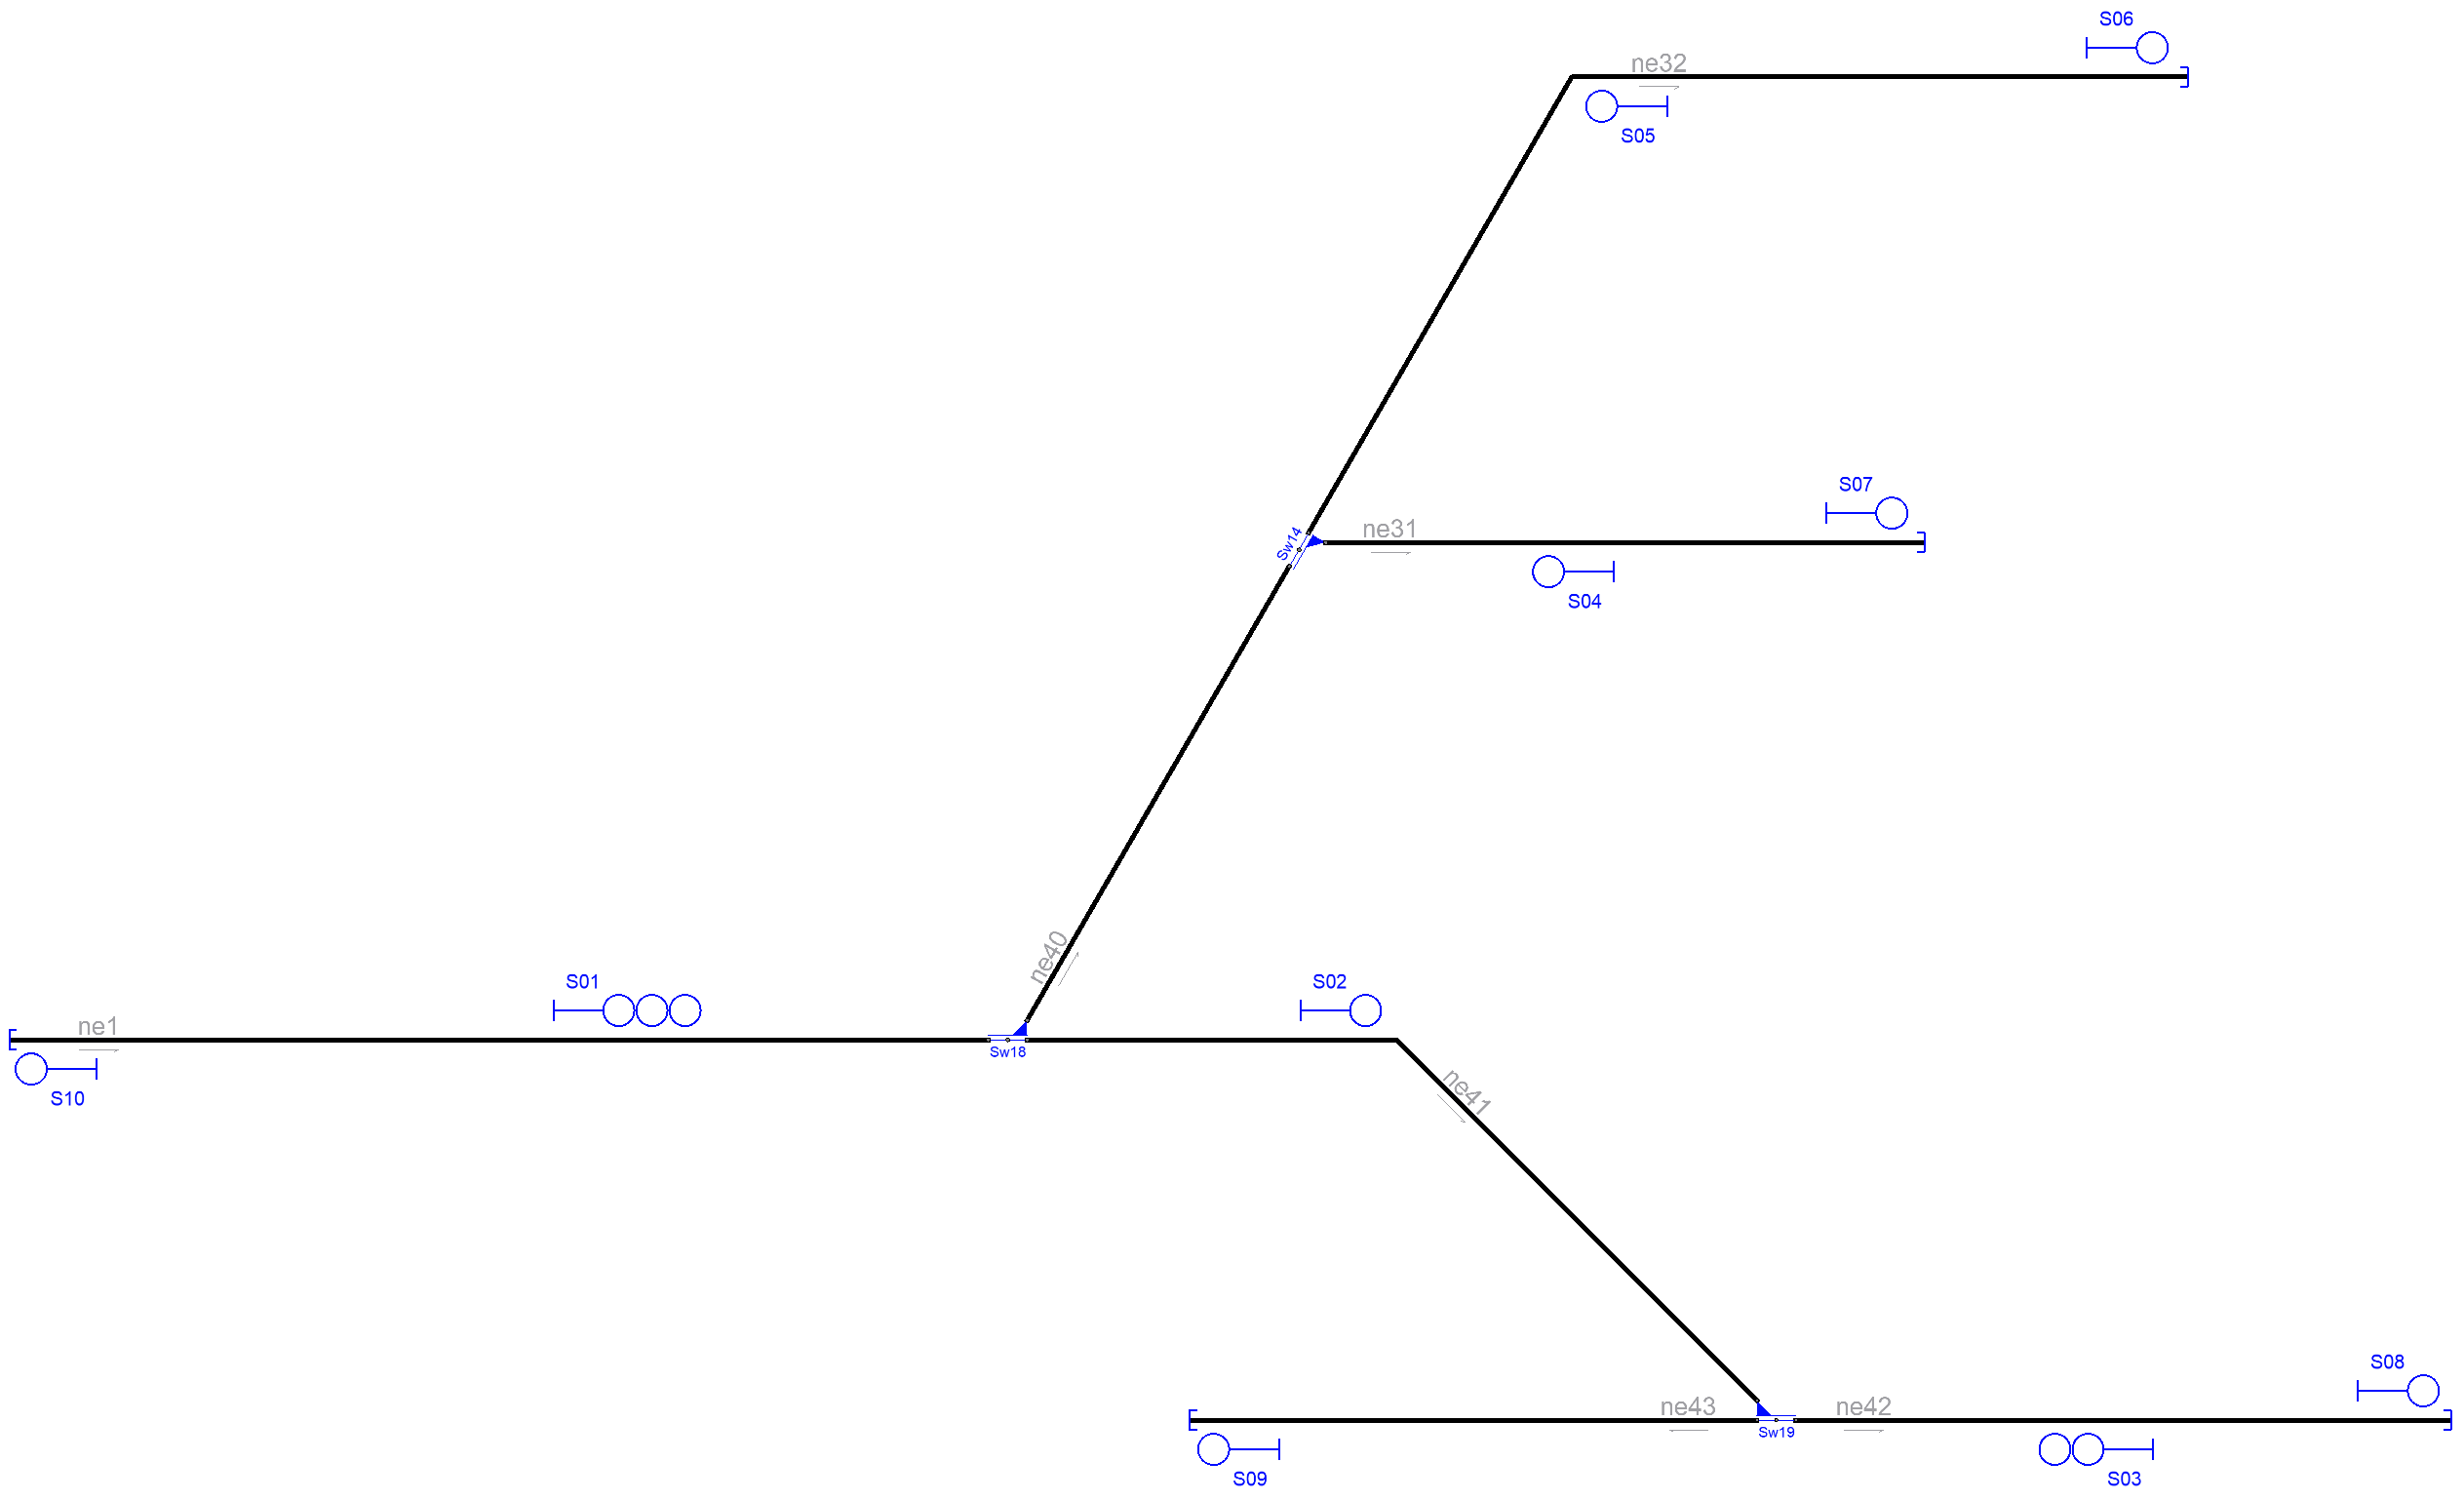
\includegraphics[width=1\textwidth]{resultados-obtenidos/ejemplo7/images/7_original.png}
    	\centering\caption{Señalamiento original del ejemplo 7.}
    	\label{fig:EJ7_2}
    \end{figure}
    
    Estas señales permiten definir hasta un máximo de 8 rutas, todas ellas detalladas en la Tabla \ref{Tab:tabla_original_7}. En una primera inspección, se puede comprobar que todos los elementos ferroviarios son alcanzados por al menos una de las rutas, en al menos una dirección. Además, todos los cambios de vías son utilizados, de forma simple o compuesta. 
    
    \begin{table}[H]
        {
        \caption{Tabla de enclavamiento original del ejemplo 7.}
        \label{Tab:tabla_original_7}
        \centering
        \resizebox{1\textwidth}{!}{
            \begin{tabular}{ c c c c c c c }
                \hline	
                    Ruta & Inicio & Final & Cambio & Plataforma & Cruce & netElement \\	
                \hline
                    R$_{01}$  & S$_{01}$ & S$_{02}$ & Sw$_{18}^{N}$ & - & - & ne$_{01}$-ne$_{41}$\\
                    R$_{02}$  & S$_{01}$ & S$_{06}$ & Sw$_{14}^{N}$+Sw$_{18}^{R}$ & - & - & ne$_{01}$-ne$_{32}$\\
                    R$_{03}$  & S$_{01}$ & S$_{07}$ & Sw$_{14}^{R}$+Sw$_{18}^{R}$ & - & - & ne$_{01}$-ne$_{31}$\\
                    R$_{04}$  & S$_{03}$ & S$_{09}$ & Sw$_{19}^{N}$ & - & - & ne$_{42}$-ne$_{43}$\\
                    R$_{05}$  & S$_{03}$ & S$_{10}$ & Sw$_{18}^{N}$+Sw$_{19}^{R}$ & - & - & ne$_{42}$-ne$_{01}$\\
                    R$_{06}$  & S$_{02}$ & S$_{08}$ & Sw$_{19}^{R}$ & - & - & ne$_{41}$-ne$_{42}$\\
                    R$_{07}$  & S$_{04}$ & S$_{10}$ & Sw$_{14}^{R}$+Sw$_{18}^{R}$ & - & - & ne$_{31}$-ne$_{01}$\\
                    R$_{08}$  & S$_{05}$ & S$_{10}$ & Sw$_{14}^{N}$+Sw$_{18}^{R}$ & - & - & ne$_{32}$-ne$_{01}$\\
                \hline
            \end{tabular}
        }
     }
    \end{table}
    
    Todas las rutas abarcan mas de un \textit{netElement}, como por ejemplo la ruta R08 que comienza en la señal S05 y finaliza en la señal S10, atravesando los \textit{netElements} ne32 y ne01, utilizando los cambios de vías Sw14 y Sw18, en posición normal y reversa respectivamente.